\documentclass[12pt]{article}
\pagestyle{empty}

%  Fonts
% \usepackage{mathpazo}
\usepackage{charter}
% \usepackage{bera}

\usepackage{amsmath}
\usepackage{amssymb}
\usepackage{amsfonts}
\usepackage{fancyhdr}
\usepackage{setspace}
\usepackage{titlesec}
\usepackage{enumitem}
\usepackage{caption}
\usepackage{booktabs}   
\usepackage{geometry}
\usepackage{hyperref}
\usepackage{float}
\usepackage{array}
\usepackage{graphicx}
\geometry{margin=1in}

\begin{document}
\section*{Introduction}
Artificial Neural Networks are fundamental tools in machine learning. The Perceptron, introduced by Frank Rosenblatt in 1957, is one of the simplest neural networks. Single Layer Perceptrons can only solve linearly separable problems, while Multi-Layer Perceptrons can handle complex, non-linear problems.

In this lab, we implement both Single Layer Perceptron and Multi-Layer Perceptron to solve logic gate problems. The AND gate is linearly separable and can be solved by Single Layer Perceptron, while the XNOR gate is non-linearly separable and requires Multi-Layer Perceptron for successful implementation.

\section*{Objectives}
The main objectives of this lab are:

\begin{enumerate}
    \item To understand the difference between linearly separable and non-linearly separable problems
    \item To implement Single Layer Perceptron for solving AND gate
    \item To implement Multi-Layer Perceptron for solving XNOR gate
    \item To demonstrate the limitation of Single Layer Perceptron on non-linear problems
    \item To compare the performance of both algorithms on logic gate implementations
    \item To gain hands-on experience with neural network programming in Python
\end{enumerate}

\section*{AND Gate Data Analysis}

\subsection*{Truth Table}
The AND gate truth table shows the expected outputs for all possible input combinations in the order used for training:

\begin{table}[H]
\centering
\caption{AND Gate Truth Table}
\renewcommand{\arraystretch}{1.5}
\begin{tabular}{|c|c|c|}
\hline
\textbf{Input A} & \textbf{Input B} & \textbf{Output (A AND B)} \\
\hline
1 & 1 & 1 \\
\hline
1 & 0 & 0 \\
\hline
0 & 1 & 0 \\
\hline
0 & 0 & 0 \\
\hline
\end{tabular}
\end{table}

\subsection*{Training Progress Overview}
The Single Layer Perceptron was trained on AND gate data for 100 epochs. The table below shows the training progress at different intervals:

\begin{table}[H]
\centering
\caption{AND Gate Perceptron Training Progress}
\renewcommand{\arraystretch}{1.5}
\begin{tabular}{|c|c|c|c|}
\hline
\textbf{Epoch} & \textbf{Weights} & \textbf{Bias} & \textbf{Predictions} \\
\hline
1 & [-0.0168, 0.0212] & -0.1818 & [0, 0, 0, 0] \\
\hline
10 & [0.1832, 0.1212] & -0.2818 & [1, 0, 0, 0] \\
\hline
20 & [0.1832, 0.1212] & -0.2818 & [1, 0, 0, 0] \\
\hline
30 & [0.1832, 0.1212] & -0.2818 & [1, 0, 0, 0] \\
\hline
40 & [0.1832, 0.1212] & -0.2818 & [1, 0, 0, 0] \\
\hline
50 & [0.1832, 0.1212] & -0.2818 & [1, 0, 0, 0] \\
\hline
60 & [0.1832, 0.1212] & -0.2818 & [1, 0, 0, 0] \\
\hline
70 & [0.1832, 0.1212] & -0.2818 & [1, 0, 0, 0] \\
\hline
80 & [0.1832, 0.1212] & -0.2818 & [1, 0, 0, 0] \\
\hline
90 & [0.1832, 0.1212] & -0.2818 & [1, 0, 0, 0] \\
\hline
100 & [0.1832, 0.1212] & -0.2818 & [1, 0, 0, 0] \\
\hline
\end{tabular}
\end{table}

\subsection*{Final Results}
\begin{table}[H]
\centering
\caption{AND Gate Final Results}
\renewcommand{\arraystretch}{1.5}
\begin{tabular}{|l|l|}
\hline
\textbf{Parameter} & \textbf{Value} \\
\hline
Final Weights & [0.1832, 0.1212] \\
\hline
Final Bias & -0.2818 \\
\hline
Final Predictions & [1, 0, 0, 0] \\
\hline
\end{tabular}
\end{table}

\subsection*{Analysis}
The training results show that the Single Layer Perceptron successfully learned the AND gate logic. After the first few epochs, the weights and bias stabilized, and the final predictions matched the expected AND gate outputs: [1, 0, 0, 0] for inputs [1,1], [1,0], [0,1], [0,0] respectively. The convergence was achieved quickly, demonstrating the linear separability of the AND gate problem.

\subsection*{Decision Boundary Visualization}
The graph below shows the decision boundary learned by the Single Layer Perceptron for the AND gate problem. The decision boundary is a straight line that separates the input space into two regions: one for class 0 (output 0) and one for class 1 (output 1).

\begin{figure}[H]
\centering
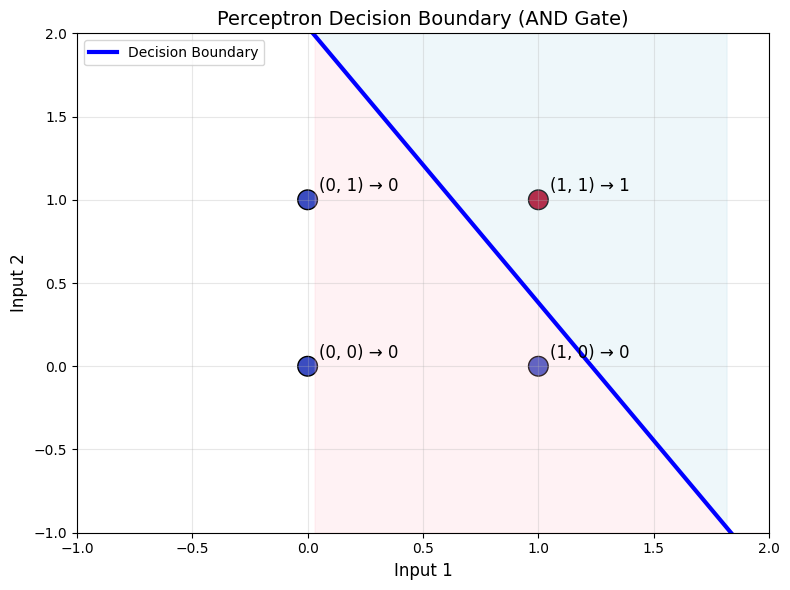
\includegraphics[width=1.0\textwidth]{and_boundary.png}
\caption{AND Gate Perceptron Decision Boundary}
\end{figure}

The decision boundary clearly separates the input points, with the point (1,1) belonging to class 1 and all other points ([1,0], [0,1], [0,0]) belonging to class 0. The linear nature of the decision boundary confirms that the AND gate is a linearly separable problem, which is why Single Layer Perceptron can successfully solve it. The weight vector [0.1832, 0.1212] and bias -0.2818 define this separating hyperplane in the 2D input space.


\section*{XNOR Gate Data Analysis}

\subsection*{Truth Table}
The XNOR gate truth table shows the expected outputs for all possible input combinations in the order used for training:

\begin{table}[H]
\centering
\caption{XNOR Gate Truth Table}
\renewcommand{\arraystretch}{1.5}
\begin{tabular}{|c|c|c|}
\hline
\textbf{Input A} & \textbf{Input B} & \textbf{Output (A XNOR B)} \\
\hline
0 & 0 & 1 \\
\hline
0 & 1 & 0 \\
\hline
1 & 0 & 0 \\
\hline
1 & 1 & 1 \\
\hline
\end{tabular}
\end{table}

\subsection*{Training Progress Overview}
The Multi-Layer Perceptron was trained on XNOR gate data for 1000 epochs. The table below shows the training progress at different intervals:

\begin{table}[H]
\centering
\caption{XNOR Gate MLP Training Progress}
\renewcommand{\arraystretch}{1.2}
\small
\begin{tabular}{|c|p{8cm}|p{6cm}|c|}
\hline
\multicolumn{1}{|c|}{\textbf{Epoch}} & \multicolumn{1}{c|}{\textbf{Layer 1→2 Weights}} & \multicolumn{1}{c|}{\textbf{Layer 2→3 Weights}} & \multicolumn{1}{c|}{\textbf{Accuracy}} \\
\hline
1 & [[-0.24, 0.89, 0.46, 0.20], [-0.68, -0.69, -0.89, 0.73]] & [[0.72], [-0.60], [-0.73], [-0.66]] & 50.00\% \\
\hline
100 & [[-1.15, 2.70, 2.74, 0.84], [-1.78, -1.82, -3.22, 1.29]] & [[1.85], [3.54], [-3.70], [-1.50]] & 100.00\% \\
\hline
200 & [[-1.47, 3.18, 2.93, 1.06], [-1.90, -2.21, -3.54, 1.40]] & [[2.22], [4.53], [-4.60], [-1.79]] & 100.00\% \\
\hline
300 & [[-1.58, 3.36, 3.01, 1.14], [-1.95, -2.35, -3.67, 1.44]] & [[2.38], [4.98], [-5.02], [-1.92]] & 100.00\% \\
\hline
400 & [[-1.65, 3.47, 3.05, 1.19], [-1.99, -2.43, -3.76, 1.47]] & [[2.49], [5.27], [-5.30], [-2.01]] & 100.00\% \\
\hline
500 & [[-1.70, 3.55, 3.08, 1.22], [-2.01, -2.49, -3.82, 1.49]] & [[2.57], [5.49], [-5.52], [-2.07]] & 100.00\% \\
\hline
600 & [[-1.73, 3.61, 3.11, 1.25], [-2.03, -2.54, -3.86, 1.50]] & [[2.63], [5.66], [-5.69], [-2.12]] & 100.00\% \\
\hline
700 & [[-1.76, 3.66, 3.13, 1.27], [-2.04, -2.57, -3.90, 1.51]] & [[2.68], [5.81], [-5.83], [-2.17]] & 100.00\% \\
\hline
800 & [[-1.78, 3.70, 3.14, 1.29], [-2.05, -2.60, -3.93, 1.52]] & [[2.73], [5.93], [-5.95], [-2.20]] & 100.00\% \\
\hline
900 & [[-1.80, 3.73, 3.15, 1.30], [-2.06, -2.62, -3.96, 1.53]] & [[2.76], [6.04], [-6.06], [-2.24]] & 100.00\% \\
\hline
1000 & [[-1.82, 3.76, 3.16, 1.32], [-2.07, -2.64, -3.98, 1.54]] & [[2.80], [6.13], [-6.15], [-2.26]] & 100.00\% \\
\hline
\end{tabular}
\end{table}



\subsection*{Final Results}
\begin{table}[H]
\centering
\caption{XNOR Gate Final Results}
\renewcommand{\arraystretch}{2.4}
\begin{tabular}{|c|c|}
\hline
\textbf{Parameter} & \textbf{Value} \\
\hline
Total Epochs & 1000 \\
\hline
Final Accuracy & 100.00\% \\
\hline
Final Predictions & [1, 0, 0, 1] \\
\hline
Expected Outputs & [1, 0, 0, 1] \\
\hline
\end{tabular}
\end{table}

\subsection*{Analysis}
The training results show that the Multi-Layer Perceptron successfully learned the XNOR gate logic. Unlike the AND gate, the XNOR gate is not linearly separable, which is why a Single Layer Perceptron cannot solve it. The MLP achieved 50\% accuracy initially (random guessing level) and then gradually improved to 100\% accuracy by epoch 100. The weights continued to evolve throughout the 1000 epochs, indicating ongoing optimization even after achieving perfect classification. The final predictions [1, 0, 0, 1] perfectly match the expected XNOR outputs for inputs [0,0], [0,1], [1,0], [1,1] respectively. This demonstrates the capability of Multi-Layer Perceptrons to solve non-linearly separable problems through the use of hidden layers and non-linear activation functions.

\subsection*{Decision Boundary Visualization}
The graph below shows the non-linear decision boundary learned by the Multi-Layer Perceptron for the XNOR gate problem. Unlike the linear decision boundary of the AND gate, the XNOR decision boundary is non-linear, consisting of two separate regions where the output is 1.


\begin{figure}[H]
\centering
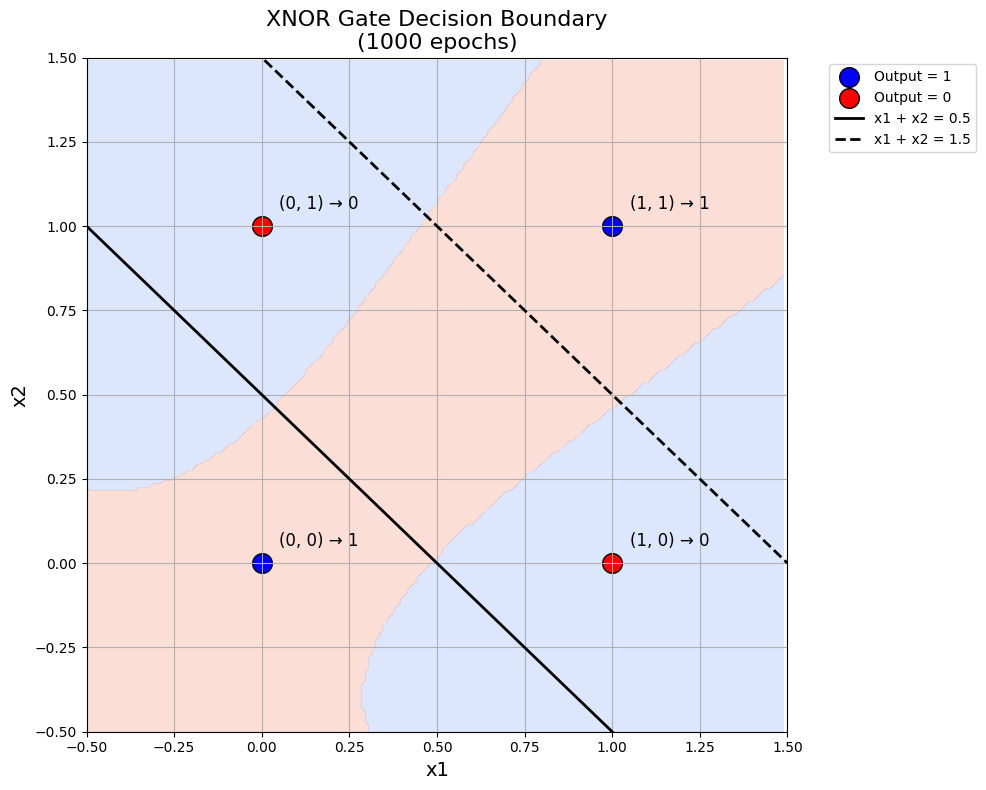
\includegraphics[width=1.0\textwidth]{xnor_boundary.png}
\caption{XNOR Gate MLP Decision Boundary}
\end{figure}

The complex, non-linear nature of the decision boundary confirms that the XNOR gate is a non-linearly separable problem. The MLP successfully creates this complex boundary through its hidden layer representations, demonstrating why multi-layer architectures are necessary for such problems.

\subsection*{MLP Architecture Visualization}
The diagram below shows the architecture of the Multi-Layer Perceptron used for solving the XNOR gate problem. The network consists of an input layer with 2 neurons (for the two inputs), a hidden layer with 4 neurons, and an output layer with 1 neuron.

\begin{figure}[H]
\centering
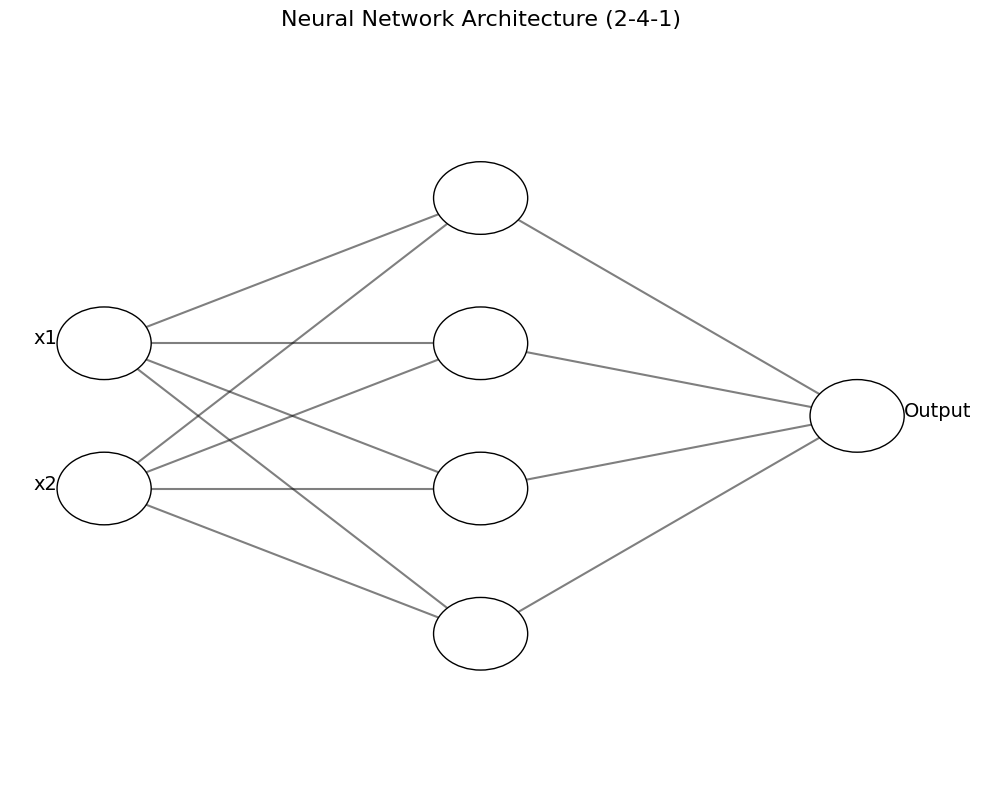
\includegraphics[width=0.8\textwidth]{xnor_neurons.png}
\caption{XNOR Gate MLP Network Architecture}
\end{figure}

The visualization illustrates how the input signals propagate through the network layers, with each connection having its own weight parameter. The hidden layer neurons apply activation functions to transform the weighted inputs, enabling the network to learn non-linear decision boundaries necessary for solving the XNOR problem.

\section*{Conclusion}
This lab demonstrated the capabilities and limitations of Single Layer Perceptrons (SLPs) and Multi-Layer Perceptrons (MLPs) through AND and XNOR gate implementations. The SLP successfully learned the linearly separable AND gate, while failing on the non-linear XNOR gate. The MLP achieved 100\% accuracy on XNOR by forming complex decision boundaries through hidden layers. Key findings include:

\begin{itemize}[noitemsep,topsep=0pt]
    \item SLPs are effective for linear problems (AND gate) but fail on non-linear cases (XNOR)
    \item MLPs solve non-linear problems via hidden layers and activation functions
    \item Decision boundary visualization confirmed the linear/non-linear separation
\end{itemize}

The results highlight the importance of network architecture selection based on problem complexity. Future work could explore deeper architectures and advanced optimization techniques.


\end{document}